%%%%%%%%%%%%%%%%%%%%%%%%%%%%%%%%%%%%%%%%%
% baposter Landscape Poster
% LaTeX Template
% Version 1.0 (11/06/13)
%
% baposter Class Created by:
% Brian Amberg (baposter@brian-amberg.de)
%
% This template has been downloaded from:
% http://www.LaTeXTemplates.com
%
% License:
% CC BY-NC-SA 3.0 (http://creativecommons.org/licenses/by-nc-sa/3.0/)
%
%%%%%%%%%%%%%%%%%%%%%%%%%%%%%%%%%%%%%%%%%

%----------------------------------------------------------------------------------------
% PACKAGES AND OTHER DOCUMENT CONFIGURATIONS
%----------------------------------------------------------------------------------------

\documentclass[landscape,a0paper,fontscale=0.285]{baposter} % Adjust the font scale/size here

\usepackage{graphicx} % Required for including images
\graphicspath{{figs/}} % Directory in which figures are stored

\usepackage{amsmath} % For typesetting math
\usepackage{amssymb} % Adds new symbols to be used in math mode

\usepackage{booktabs} % Top and bottom rules for tables
\usepackage{enumitem} % Used to reduce itemize/enumerate spacing
\usepackage{palatino} % Use the Palatino font
\usepackage[font=small,labelfont=bf]{caption} % Required for specifying captions to tables and figures

\usepackage{multicol} % Required for multiple columns
\setlength{\columnsep}{1.5em} % Slightly increase the space between columns
\setlength{\columnseprule}{0mm} % No horizontal rule between columns

\newcommand{\compresslist}{ % Define a command to reduce spacing within itemize enumerate environments, this is used right after \begin{itemize} or \begin{enumerate}
\setlength{\itemsep}{1pt}
\setlength{\parskip}{0pt}
\setlength{\parsep}{0pt}
}

\definecolor{lightblue}{rgb}{0.145,0.6666,1} % Defines the color used for content box headers

\begin{document}

\begin{poster}
{
headerborder=closed, % Adds a border around the header of content boxes
colspacing=1em, % Column spacing
bgColorOne=white, % Background color for the gradient on the left side of the poster
bgColorTwo=white, % Background color for the gradient on the right side of the poster
borderColor=lightblue, % Border color
headerColorOne=black, % Background color for the header in the content boxes (left side)
headerColorTwo=lightblue, % Background color for the header in the content boxes (right side)
headerFontColor=white, % Text color for the header text in the content boxes
boxColorOne=white, % Background color of the content boxes
textborder=roundedleft, % Format of the border around content boxes, can be: none, bars, coils, triangles, rectangle, rounded, roundedsmall, roundedright or faded
eyecatcher=true, % Set to false for ignoring the left logo in the title and move the title left
headerheight=0.1\textheight, % Height of the header
headershape=roundedright, % Specify the rounded corner in the content box headers, can be: rectangle, small-rounded, roundedright, roundedleft or rounded
headerfont=\Large\bf\textsc, % Large, bold and sans serif font in the headers of content boxes
%textfont={\setlength{\parindent}{1.5em}}, % Uncomment for paragraph indentation
linewidth=2pt % Width of the border lines around content boxes
}
%-------------------------------------------------------------------------------
% TITLE SECTION
%-------------------------------------------------------------------------------
%
{
\includegraphics[height=7em]{logo_cal.jpg}} % university/lab logo on the left
{\bf\textsc{Optimal Prediction with SuperLearner}\vspace{0.5em}} % Poster title
{\textsc{\{ Nima Hejazi \& Alan Hubbard \} \hspace{12pt} Division of Biostatistics, UC Berkeley}}
  % Author names and institution
{
\includegraphics[height=9em]{logo_sph.jpg}} % university/lab logo on the right

%-------------------------------------------------------------------------------
% OVERVIEW
%-------------------------------------------------------------------------------

\headerbox{Overview}{name=overview,column=0,row=0}{

\begin{enumerate}\compresslist
\item This analysis seeks to generate optimal predictions for 5 genomic
  covariates across 67 sample observations, nearly evenly distributed across 5
  \textit{"knockout"} genotypes.
\item \textbf{Uninformative censoring:} the competition rules indicate that
  missingness was artificially introduced; this greatly simplifies the missing
  data problem to be solved via prediction methods.
\item Rather than use a single machine learning algorithm to estimate the
  missing values in the data set, a weighted combination of a library of
  learning algorithms is used to generate provably optimal predictions.
\item While the theory underlying the SuperLearner methodology is quite rich, at
  its core, the method simply uses cross-validation to rank learning algorithms
  within a provided library according to a meta-learner, building a weighted
  combination of learning algorithms for prediction.
\end{enumerate}

\vspace{0.3em} % When there are two boxes, some whitespace may need to be added
               % if the one on the right has more content
}

%-------------------------------------------------------------------------------
% INTRODUCTION
%-------------------------------------------------------------------------------

\headerbox{Introduction}{name=introduction,column=1,row=0,bottomaligned=overview}{

\begin{itemize}
\item The goal of this prediction challenge is to infer the withheld values of a
  single genomic covariate for a subset of individuals from 5 randomly selected
  "knock-out" conditions in the full data set provided.
\item In order to predict the missing values in a \textit{provably optimal}
  manner, this analysis relies on the SuperLearner algorithm, to generate
  asymptotically optimal prediction.
\item The problem of overfitting with the individual (and ensemble) learners is
  avoided by employing V-fold cross-validation (where $V = 10$ in the results
  presented).
\item The 5 genomic covariates that we provide predicted values for all have
  continuous measurements, thus, we use the squared error (L2) loss function
  with SuperLearner.
\end{itemize}
}

%-------------------------------------------------------------------------------
% RESULTS 2
%-------------------------------------------------------------------------------

\headerbox{Results II}{name=results,column=2,span=2,row=0}{

\begin{multicols}{2}

\begin{center}
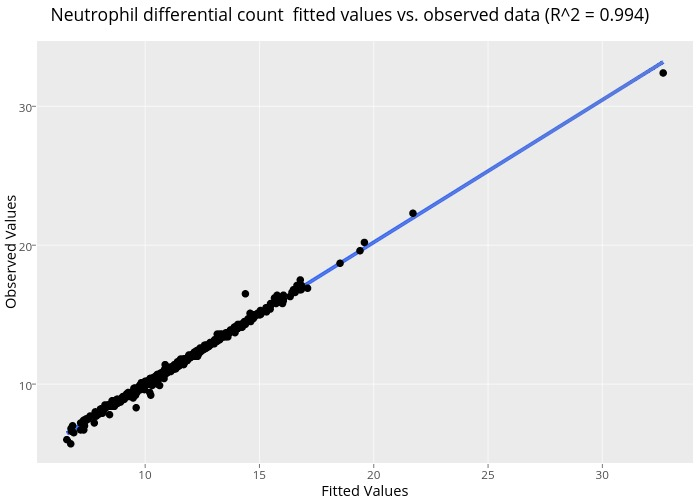
\includegraphics[scale=0.25]{covar2_neutrophils}
\captionof{figure}{fitted vs true values for neutrophils}
\end{center}

\begin{center}
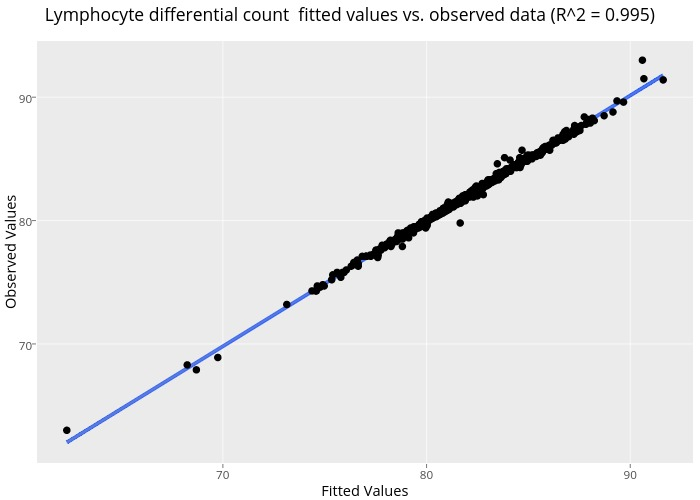
\includegraphics[scale=0.25]{covar3_lymphocytes}
\captionof{figure}{fitted vs true values for lymphocytes}
\end{center}

\end{multicols}

%------------------------------------------------

\begin{multicols}{2}

\begin{center}
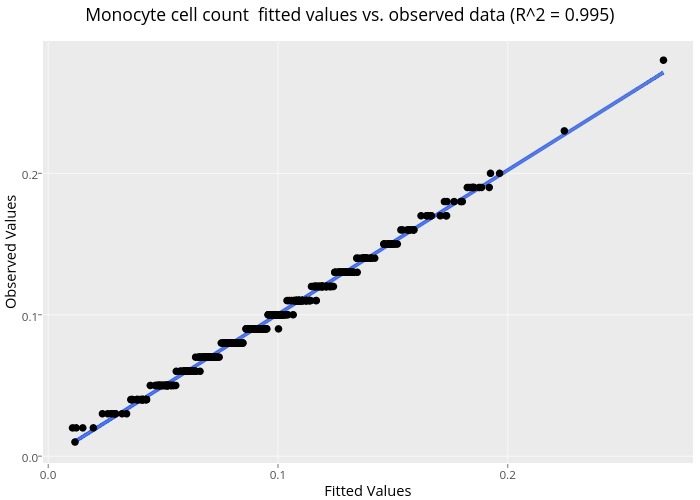
\includegraphics[scale=0.25]{covar4_monocytes}
\captionof{figure}{fitted vs true values for monocytes}
\end{center}

\begin{center}
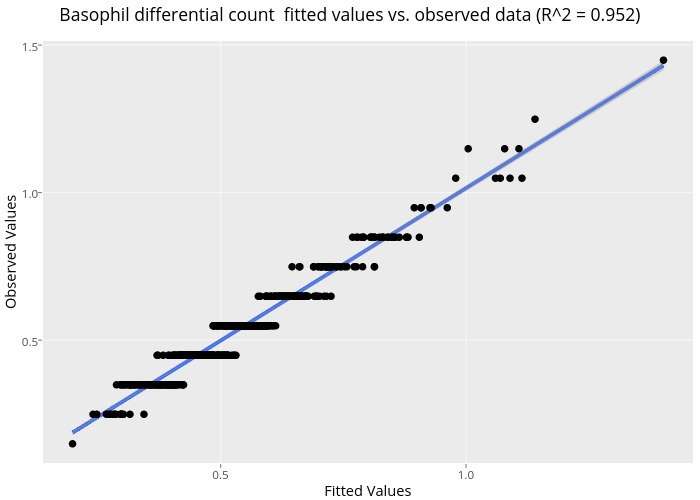
\includegraphics[scale=0.25]{covar5_basophils}
\captionof{figure}{fitted vs true values for basophils}
\end{center}

\end{multicols}
}

%-------------------------------------------------------------------------------
% REFERENCES
%-------------------------------------------------------------------------------

\headerbox{References}{name=references,column=2,above=bottom}{
\renewcommand{\section}[2]{\vskip 0.05em} % remove "References" section title
\nocite{*} % Insert publications even if they are not cited in the poster
\tiny{ % Reduce the font size in this block
\bibliographystyle{unsrt}
\bibliography{conference_poster}
}}


%-------------------------------------------------------------------------------
% CONTACT INFORMATION
%-------------------------------------------------------------------------------

\headerbox{Contact Information}{name=contact,column=3,aligned=references,above=bottom}{
  % This block is as tall as the references block

\begin{description}\compresslist
\item[Web] \small http://nimahejazi.org \& hubbard.berkeley.edu \\
\item[Email] \small nhejazi@berkeley.edu \& hubbard@berkeley.edu
\end{description}
}

%-------------------------------------------------------------------------------
% CONCLUSION
%-------------------------------------------------------------------------------

\headerbox{Conclusion}{name=conclusion,column=2,span=2,row=0,below=results,above=references}{

\begin{multicols}{2}

\begin{center}
\vspace*{-0.51cm}

\includegraphics[scale=0.285]{genes_correlationGraph.pdf}
\vspace{-1.8em}
\captionof{figure}{Graph of Correlation Structure}
\end{center}

%------------------------------------------------

\begin{itemize}
\item In order to visualize the relationship between the genomic covariates in
  the observed data set, a graph is generated from the correlation matrix.
\item We hold that a predictive analysis \textbf{\textit{does not target causal
  parameters}}. Thus, we refrain from providing a causal graph in our work.
\item SuperLearner provides asymptotically optimal prediction, and our results
  display MSE values that substantiate this claim.
\end{itemize}

\end{multicols}
}

%-------------------------------------------------------------------------------
% METHODS
%-------------------------------------------------------------------------------

\headerbox{Methodology}{name=method,column=0,below=overview,bottomaligned=references}{
  % This block's bottom aligns with the bottom of the conclusion block

The \textbf{SuperLearner} method works as follows:

\vspace{-0.2em}

\begin{itemize}\compresslist
\item Start by defining a base library of L learners:
  $\Psi^{1}, \dots, \Psi^{L}$ to be used within SuperLearner.
\item Specify a meta-learning method ($\Phi$), used to evaluate the base
  learners.
\item Use V-fold cross validation in each estimation step ($V = 10$ in our case)
  to protect against overfitting and evaluate learners.
\item Each base learner is used to generate fitted values for the training fold,
  generating a new matrix of subset-specific fits.
\item Then, the meta-learner is used to find the optimal combination of these
  fits.
\end{itemize}

In the analysis for this competition, we have used:

\vspace{-0.2em}

\begin{itemize}\compresslist
\item The full data set, iteratively predicting values for the 5 genomic
  covariates of interest
\item In each run of SuperLearner, indicator variables are used to impute the
  missing values remaining in the training set.
\end{itemize}
}

%-------------------------------------------------------------------------------
% RESULTS 1
%-------------------------------------------------------------------------------

\headerbox{Results I}{name=results2,column=1,below=overview,bottomaligned=references}{
  % This block's bottom aligns with the bottom of the conclusion block

To assess the performance of SuperLearner, we apply the mean squared error,
discounting observations with missing data in each of the 5 genomic covariates
of interest. \\

That is, for each covariate $j$, observations with missing values in $y_{j}$,
and corresponding fitted values in $\hat{y_{j}}$, are removed, then MSE is
applied:
$$ MSE_{j} = \frac{1}{n_{j}} \sum_{i = 1}^{n_{j}} (\hat{y_{j}} - y_{j})^{2} $$

\begin{center}
\begin{tabular}{l l}
\toprule
\textbf{Covariate} & \textbf{MSE}\\
\midrule
RBC Distribution Width & 0.00004096 \\
Neutrophil Differential Count & 0.00846919 \\
Lymphcyte Differential Count & 0.06623846 \\
Monocyte Cell Count & 0.00005010 \\
Basophil Differential Count & 0.00007293 \\
\bottomrule
\end{tabular}
\captionof{table}{"Competition" Covariates with MSE}
\end{center}
}

%-------------------------------------------------------------------------------

\end{poster}

\end{document}
